\chapter{Metodologia}
\label{chap:metodologia}

\section{MLP (Perceptron Multicamadas)}

Como é mostrado na Figura \ref{fig:subfigura1}, uma Rede Neural Multicamadas (MLP – \textit{MultiLayer Perceptron})
é formada por um conjunto de neurônios, também conhecidos como
\textit{Perceptrons}. Uma MLP consiste em uma camada de entrada, juntamente com uma ou mais camadas ocultas.
No processo de treinamento, é empregada uma técnica chamada retropropagação (\textit{backpropagation}), que
ocorre em duas fases distintas: a propagação para frente (\textit{forward}) e a retropropagação propriamente
dita (\textit{backward}), assim como ilustra a Figura \ref{fig:subfigura2}. Durante a propagação para frente, os dados são passados pela rede, camada por camada,
permitindo que as saídas da rede sejam calculadas. Em seguida, durante a fase de retropropagação, os
erros entre as saídas previstas e os valores reais são calculados e propagados de volta através da rede,
ajustando os pesos das conexões para minimizar esses erros. Esse processo iterativo é fundamental para o
treinamento eficaz de uma MLP, permitindo que ela aprenda e se adapte \cite{su12114776}.  

\begin{figure}[h]
    \centering
    \caption{Estrutura e atividade de uma rede MLP, imagens de \cite{su12114776}.}
    \begin{subfigure}{0.4\textwidth}
      \centering
      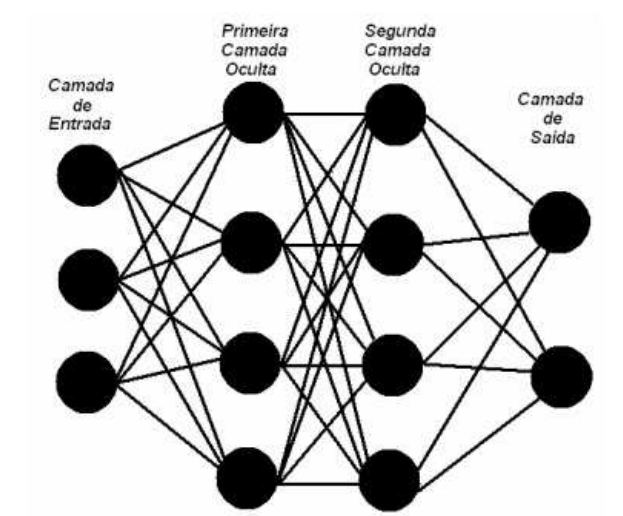
\includegraphics[width=\linewidth]{figuras/MLP/rede_MLP.png}
      \caption{Camadas de uma MLP.}
      \label{fig:subfigura1}
    \end{subfigure}
    \hspace{5mm}
    \begin{subfigure}{0.45\textwidth}
      \centering
      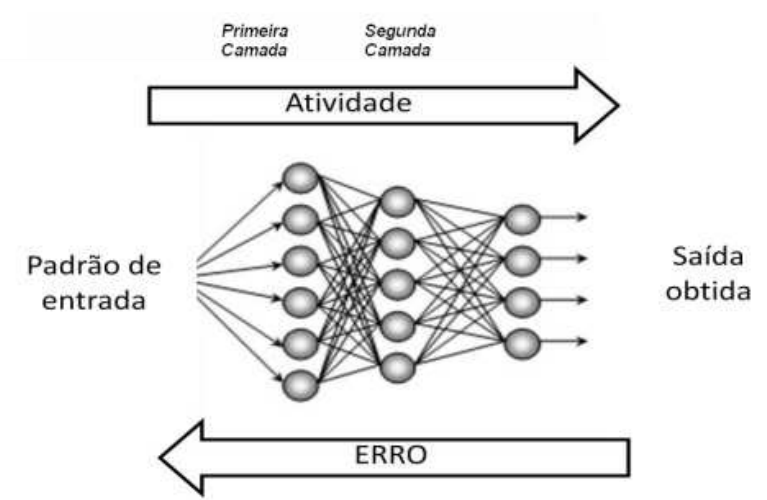
\includegraphics[width=\linewidth]{figuras/MLP/atividade_MLP.png}
      \caption{\textit{Forward} e \textit{backward} em uma rede MLP.}
      \label{fig:subfigura2}
    \end{subfigure}
    \label{fig:subfiguras}
  \end{figure}

\section{Naive Bayes}

\textit{Naive} Bayes é um método de classificação e tem como base o teorema de Bayes. Este método
gera uma tabela de probabilidades utilizadas para classificar os dados, as \textit{features} dos 
dados são analisadas de forma independente, por isso o nome \textit{Naive}, que significa
ingênuo. A Equação \ref{eq:bayes}, abaixo, descreve o funcionamento desse método de classificação \cite{BattaMahesh2018}.

\begin{itemize}
    \item Teorema de Bayes:
    \begin{equation}
        P(c|x) = P(c)P(x|c)/P(x)
        \label{eq:bayes}
    \end{equation}

    \begin{itemize}
        \item $P(c|x)$: \textbf{Probabilidade Posterior}, probabilidade do dado $(x)$ pertencer a classe $(c)$;
        \item $P(c)$: \textbf{Probabilidade Anterior}, probabilidade da classe $(c)$ ocorrer antes do dado $(x)$;
        \item $P(x|c)$: \textbf{Verossimilhança}, caso a classe $(c)$ seja verdadeira, a probabilidade $(x)$ ocorrer em $(c)$;
        \item $P(x)$: \textbf{Probabilidade marginal x}, probabilidade de $(x)$ ser observado idenpendente de $(c)$.
    \end{itemize}
\end{itemize}

% Ao finalizar todas as verificações para todas as evidências, ou seja dados $(x)$, presentes no dataset uma tabela de probabilidades 
% é formada classificando os dados.



\section{Support Vector Machine (SVM)}

É uma técnica supervisionada utilizada para classificação e regressão. Esse método cria um vetor que divide as classes
com margens, para minimizar os erros \cite{BattaMahesh2018}. A Figura \ref{fig:SVM_1}, mostra como a divisão de classes
acontece.

\begin{figure}[h]
    \centering
    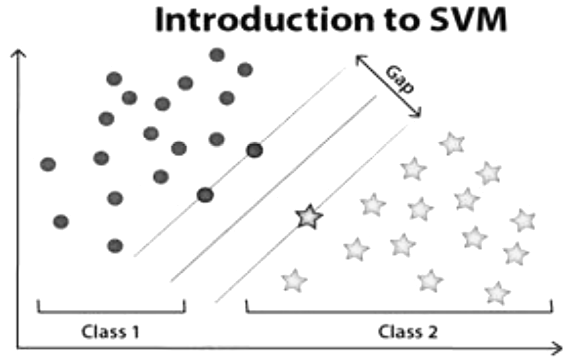
\includegraphics[width=8cm]{figuras/SVM/SVM_1.png}
    \caption{Divisão de classes por vetores, Figura de \cite{BattaMahesh2018}.}
    \label{fig:SVM_1}
\end{figure}

\textit{Kernel} é uma função responsável por calcular a similaridade entre pares de conjuntos, as entradas, e o resultado são números
escalares que representam o grau semelhança entre as amostras \cite{noronha2016implementaccao}. Uma função é chamada de \textit{kernel} quando satisfaz as condições do teorema de mercer. 
De acordo com esse teorema se a matiz k é positivamente definida, ou seja k é a matriz do produto interno dos dados de entrada \cite{falcao2017aplicaccao}.

\subsection{kernel RBF}

\begin{equation}
  exp\left (-\frac{||xi - xj||^2}{2\alpha^2}  \right )
  \label{eq:polinK}
\end{equation}

\subsection{kernel Polinomial}

Kernel Polinomial calcula a similaridade dos pares por meio de uma função polinomial. É amplamente utilizado, pois possui bom desempenho com relação ao processamento de linguagem natural. Também é 
possível, através dessa função, classificar problemas não linearmente separados \cite{noronha2016implementaccao}. 

\begin{equation}
  [(xi\cdot xj) + 1]^p
  \label{eq:polinK}
\end{equation}


\subsection{kernel Linear}
oi oio oi